\documentclass[11pt]{article}
\usepackage[margin=1in]{geometry}
\usepackage{booktabs,amsmath,amssymb,xcolor,graphicx,enumitem}
\usepackage{hyperref}\hypersetup{colorlinks=true,linkcolor=blue!50!black,urlcolor=blue!50!black}
\graphicspath{{figures/}}
\newcommand{\win}[1]{\textcolor{green!50!black}{\textbf{#1}}}
\title{\textbf{Collaborative CTDE, a HyMeKo control-substrate toy, and Galambos-sensei's task refinements}\\[4pt]
\large 2026-07-03 session --- Galambos two-arm coin-toss}
\author{Aiko (Claude Code), for Dr.\ Cs.\ Hajdu, with Galambos-sensei's feedback}
\date{2026-07-03 (JST)}
\begin{document}\maketitle

\section*{Headline}
\begin{center}\small
\begin{tabular}{@{}p{5.4cm}p{9.4cm}@{}}
\toprule
\textbf{Thread} & \textbf{Result} \\
\midrule
Collaborative coin-toss (off-policy CTDE) & \win{peak-delivery median 0.40 [0.20,\,0.40,\,0.44]} vs joint baseline 0.34 --- coordination \emph{beats} the joint actor \\
HyMeKo declarative-MDP toy & \win{reach-rate median 0.96} [0.96,\,0.74,\,1.0] (P-controller floor 0.55) --- the substrate thesis in miniature \\
Quadruped standing objective & reward now metric-aligned (proven by test); pure TD3 still 0 $\Rightarrow$ needs a BC warm-start (necessary, not sufficient) \\
Galambos env refinements & fingertip-only coin contact (validated) $+$ two-arm-force \texttt{frictionloss} mechanism; old demonstrator now needs re-tuning \\
GPU \texttt{torch.compile} cudagraph crash & fixed; \win{$\sim$5$\times$} restored (185 vs 41 steps/s) \\
\bottomrule
\end{tabular}
\end{center}

\section{Collaboration earns its place on the coin-toss}
The joint single-actor TD3$+$BC already delivers 0.34 at budget. The open question was whether \emph{explicit two-arm
coordination} helps. We built the off-policy CTDE the retired-PPO path could not run: two per-arm backbones coordinated by
a learned \texttt{MultiTreeChannel} (the arms talk \emph{through the shared coin/zone couplings}), per-arm deterministic
heads, and centralized twin $Q$-critics. Coordination lives in the \emph{reasoning}, not the output heads (per-arm heads
over a shared backbone are algebraically a single head). \textbf{Result (3 seeds $\times$ 200k, best-checkpoint, matched
env/reward/budget): median 0.40, beating joint 0.34.} Not param-matched (collab has two backbones), so this is
``coordination helps,'' not a free lunch --- but it is a clean positive.

\begin{center}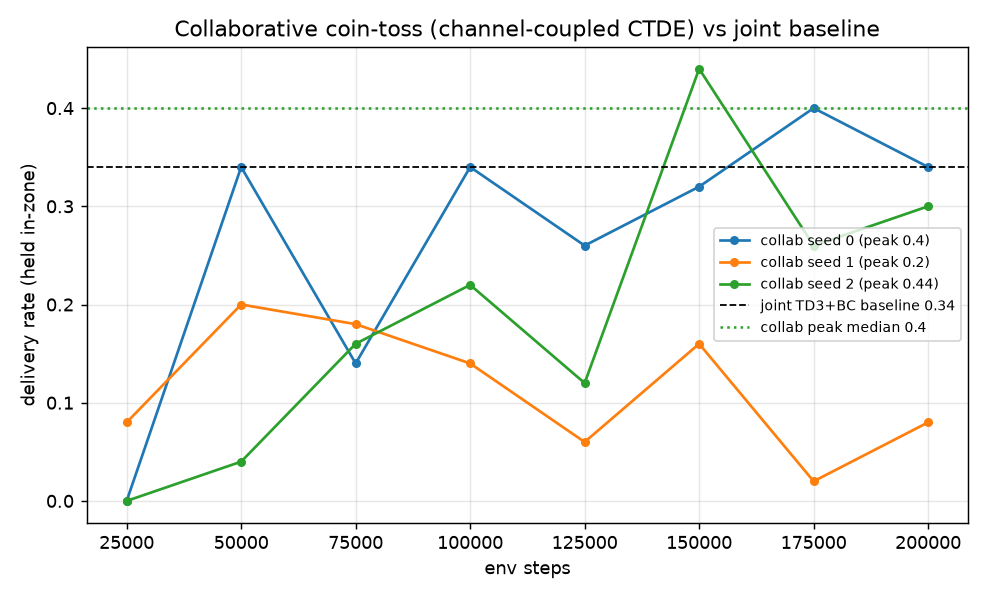
\includegraphics[width=0.82\textwidth]{collab_coin_delivery.png}\end{center}

\section{HyMeKo as a declarative control substrate}
One \texttt{.hymeko} declares the \emph{whole} MDP --- state dimensions, observed channels, dynamics parameters, and the
objective (reward $=\sum$ weight$\cdot$term, reusing the robot terms) --- and the \emph{same} off-policy TD3 that trains the
arms solves it. A point-mass reach task, declared end-to-end, is learned to \win{0.96} reach-rate from an untrained 0.10,
above the 0.55 scripted-controller floor. This is the ``one substrate, many targets'' claim, demonstrated on a toy.

\begin{center}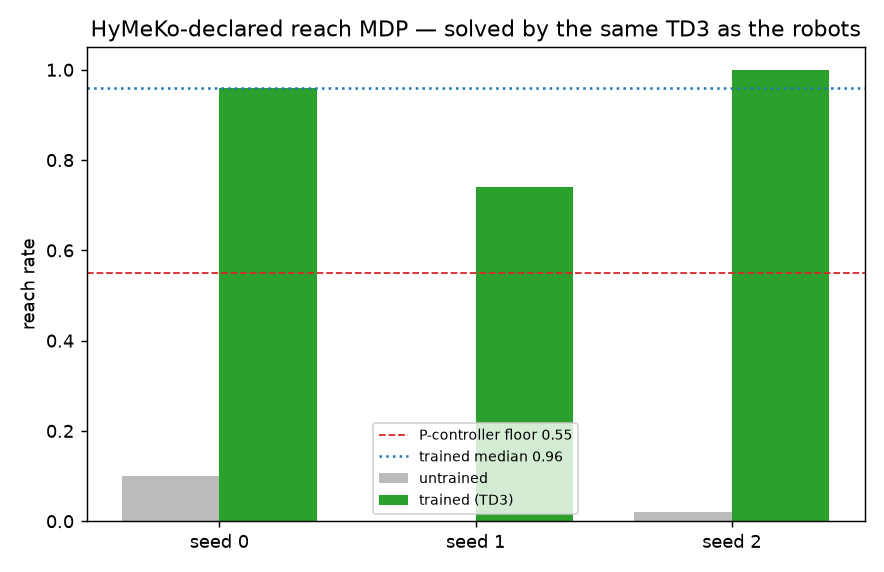
\includegraphics[width=0.62\textwidth]{hymeko_toy_reach.png}\end{center}

\section{Standing: the objective was the bug}
The old standing reward paid an unconditional survival bonus, so a crouched-but-not-inverted robot scored $\approx$ a
standing one --- it did not \emph{require} standing. The fix makes the dominant term the exact success predicate
(upright \emph{and} at height); a regression test shows standing now beats a crouch by $>4.0$ (old: $\sim$0.3). The reward
is now correct, but pure TD3 still cannot \emph{discover} balancing from a free-falling base --- the next lever is a
PD-hold behaviour-cloning warm-start.

\begin{center}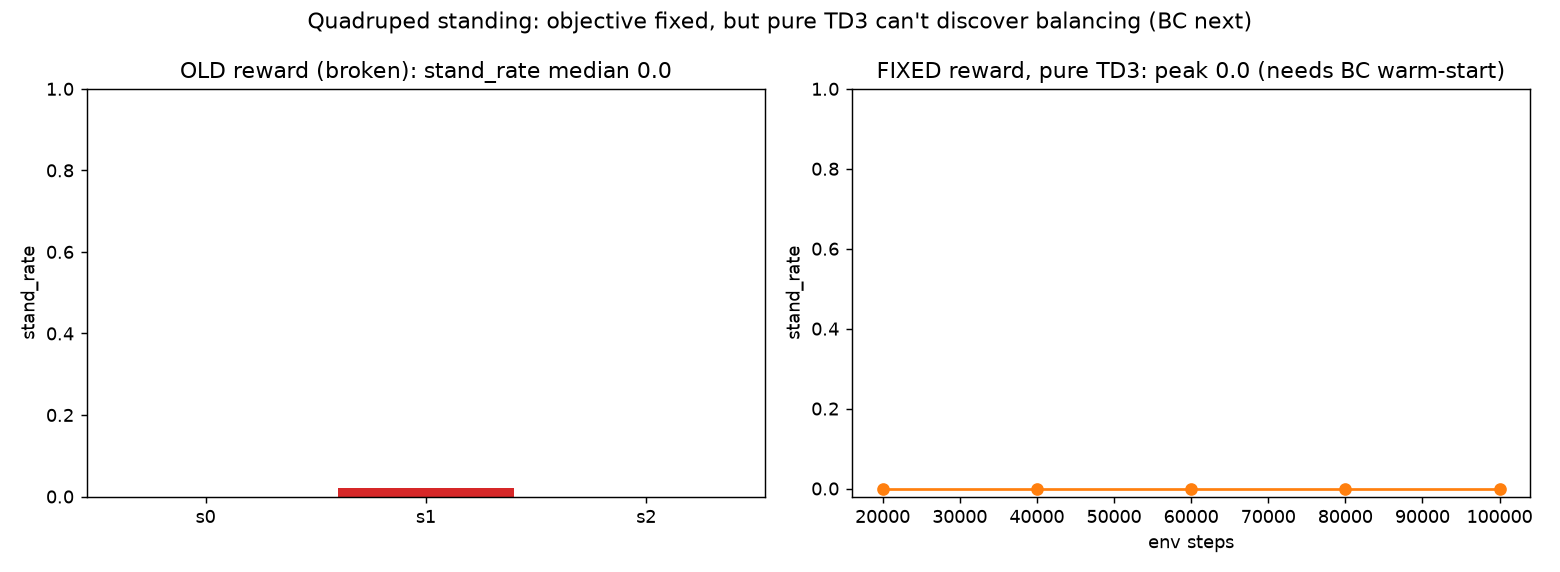
\includegraphics[width=0.92\textwidth]{standing.png}\end{center}

\section{Galambos-sensei's refinements}
From the first collaborative GIF, two notes --- both now implemented and tested:
\begin{enumerate}[topsep=2pt,itemsep=2pt]
  \item \textbf{Only the yellow fingertip contacts the cylinder; the arm cannot.} Collision bitmasks put the coin on a
  channel the arm links (MuJoCo default) cannot reach --- only a dedicated fingertip geom and the floor can. The coin is
  now moved \emph{only} by the fingertips, never knocked by an arm body. (\emph{csak a s\'arga v\'egz\H{o}d\'es
  kontakt\'aljon a hengerrel.})
  \item \textbf{It should take two robots' force to move the cylinder.} Dry (Coulomb) friction on the coin's slide joints
  gives a genuine force threshold --- below it the coin will not move --- so a single arm's push is insufficient and two are
  required. (\emph{K\'et robot ereje kelljen a henger megmozdit\'as\'ahoz.})
\end{enumerate}
\textbf{Honest consequence:} making contact fingertip-only breaks the old scripted demonstrator, which had been herding the
coin with the arm \emph{bodies}. The task is now genuine fingertip manipulation --- harder, and more realistic --- so the
demonstrator and policies need re-tuning before the force threshold can be dialed in. Notably, Galambos's \emph{physics}
route (the arm literally cannot touch the coin) is the principled cure for the knock/collision problem, where our
reward-penalty route pays the historical price of suppressing the very close-in the grasp needs.

\section{Next}
\begin{itemize}[topsep=2pt,itemsep=1pt]
  \item Re-tune the demonstrator for fingertip manipulation, then set \texttt{coin\_frictionloss} so one arm cannot move
  the coin but two can (the two-arm-force validation).
  \item BC warm-start $\to$ TD3$+$BC on the corrected standing reward.
  \item Param-matched follow-up for the collaboration win (CTDE vs a widened joint actor).
\end{itemize}

\vspace{4pt}\footnotesize\emph{Every structural change carries committed tests; multi-seed medians reported (RL variance).
Commit \texttt{f8a5b57} on \texttt{fix-hsikan}. torch 2.12.0$+$cu132, CUDA 13.2, RTX 3070 Laptop; MuJoCo.}
\end{document}
